%----------------------------------------------------------------------
% Problem 3

\begingroup
\allowdisplaybreaks

\newpage
\section*{Problem 3}

\begin{figure}[h]
	\centering
	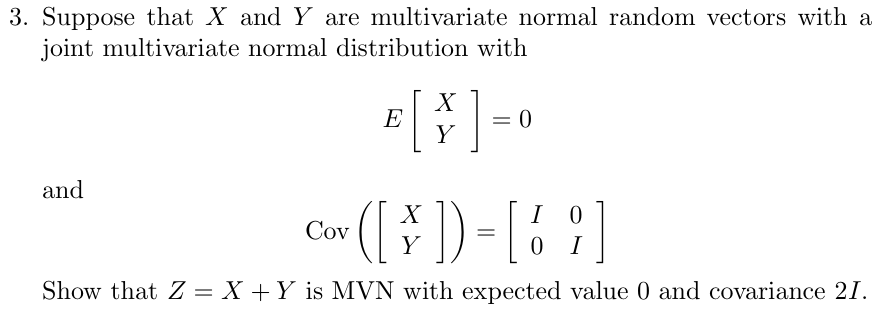
\includegraphics[width=0.8\textwidth]{./images/prob3_statement.png}
\end{figure}

\subsection*{Solution}

Given the problem statement, let random vectors $\bv{X}$ and $\bv{Y}$ contain the same number of elements and each vector is identically distributed such that

\begin{align*}
	\bv{X},\,\bv{Y} \sim \textrm{N}\left(0,\,I\right)
\end{align*}

Given the new random vector $\bv{Z} = \bv{X} + \bv{Y}$, the expected value of $\bv{Z}$ is

\begin{align*}
	\E{\bv{Z}} &= \E{\bv{X} + \bv{Y}} \\
	\\
	&= \E{\bv{X}} + \E{\bv{Y}} \\
	\\
	&= \bv{0} + \bv{0} \\
	\\
	&= \bv{0} \,\,\,\,\, \textcolor{green}{\checkmark}
\end{align*}

\textcolor{red}{Not sure if "covariance" is a typo, I suspect it should be "variance"? If so...}

The variance of $\bv{Z}$ is

\begin{align*}
	\Var{\bv{Z}} &= \Var{\bv{X} + \bv{Y}} \\
	\\
	&= \Var{\bv{X}} + \Var{\bv{Y}} + 2\Cov{\bv{X},\bv{Y}}
\end{align*}

Given the problem statement, the covariance of the concatenation of random vectors $\bv{X}$ and $\bv{Y}$ shows that these two random vectors are independent of each other. Therefore

\begin{align*}
	\Var{\bv{X}} + \Var{\bv{Y}} + 2\Cov{\bv{X},\bv{Y}} &= \Var{\bv{X}} + \Var{\bv{Y}} + 0 \\
	\\
	&= I + I \\
	\\
	&= 2I \,\,\,\,\, \textcolor{green}{\checkmark}
\end{align*} 



